\chapter{Online Deployment}%
\label{sec:operation}



This section reports the \rnn{} operation in both 2017
(Section~\ref{ssec:2017_ringer_operation}) and 2018
(Section~\ref{ssec:2018_ringer_operation}) data acquisition periods. The operation efficiencies
are computed with respect to offline electrons, as indicated in
Section~\ref{ssec:dataset}\footnote{For efficiency measurements in this section,
	fake electrons are selected always employing \veto\vloose{} offline likelihood
	working point.}. Firstly, we detail the algorithm cycle during Run~2
(Section~\ref{ssec:run2_rnn_cycle}).

\section{Run~2 \rnn{} Cycle}\label{ssec:run2_rnn_cycle}

During the Run 2, the actual \rnn{} implementation
%The \rnn cycle 
can be partitioned into four chronological stages:

\begin{enumerate}[i]
  \item A development stage up to early 2017, where the \rnn{}
      potential was estimated from trigger emulation and data reprocessing;
  \item The commissioning stage (\SI{5.4}{\per\femto\barn}) occurred in
      early 2017 runs, where all primary
      triggers were duplicated with either the \rnn{} or cut-based algorithms
      operating in the \fastcalo{};
  \item The operation of the method as the baseline trigger, which occurred after 2017 Technical Stop 1 (TSP1). For
    monitoring purposes, and to allow precise statistical evaluation of eventual
    disagreements between the \fastcalo{} methods from an offline
    perspective (Section~\ref{sec:off_ana}), a duplicated trigger pair, i.e.
    with and without \rnn{}, was kept operating unprescaled during this period
    (\SI{39.0}{\per\femto\barn}). Here, we compare the efficiencies of the
    duplicated triggers in 2017 (Section~\ref{ssec:2017_ringer_operation});
  \item Finally, the duplicated trigger was removed for 2018 operation.
    Therefore, we evaluate 2018 \rnn{} operation relying on a comparison with
    2017 efficiency in Section~\ref{ssec:2018_ringer_operation}.
\end{enumerate}

\section{2017 Operation}\label{ssec:2017_ringer_operation}

% FIXME Don't forget that there are some of these plots that were already
% approved.

%A backup trigger ($\text{e28\_lhtight\_nod0\_ivarloose}$) was employed for
A backup trigger ($E_T > 28$ GeV isolated with Tight selection and without the \rnn{}) was employed for
monitoring purposes after the TS1. During the monitoring process, a similar
operation of both triggers was observed in terms of signal efficiency using the
integrated luminosity along the period, as shown in
Figure~\ref{fig:e28_triggers}. The trigger
turn-on curves exhibit similar profile. In $\eta$, \rnn{} shows a reasonably symmetric
profile with respect to positive and negative $\eta$, while a
\SI{3}{\%} efficiency loss is observed at $-2.01<\eta<-1.81$\footnote{The cause for this efficiency loss is unknown, but we expect it to be caused by a change in either one or more of the ratio profiles reconstructed by the FastCalo.}. In addition, a difference of about
half to one percentage point may be observed in $\eta$ regions (crack regions) with deterioration in the calorimeter
response ($1.37 < \abseta < 1.52$ and $2.37 < \abseta < 2.45$). Besides
aforementioned points, overall efficiency fluctuations are smaller than a few
per-mill. Although a slight more prominent efficiency loss with respect to
\avgmu{} is observed in Figure~\ref{fig:e28_comp_mu} for the \rnn{} trigger, the
electron efficiency was kept nearly the same. Such loss occurs after the
linear threshold correction limit that was employed during 2017 ($\avgmu=40$).

Other important triggers were assessed by comparing the trigger efficiencies on
2017 data collected before and after switching to the \rnn{} algorithms.  As it can be
observed in Figure~\ref{fig:2017_ts1}, the electron efficiency was also kept
nearly unchanged for relevant single electron triggers. Note that results in
this plot are computed with two different data taking periods (with or
without the \rnn{} algorithm). The e17\_lhvloose\_nod0 trigger shows the
efficiency in the lowest-energy-threshold 
% efficiency of the legs in the lowest-energy-threshold 
unprescaled two electron trigger.
Similar behavior was observed during data collection for all monitored triggers.


\begin{figure}[h!tb]
  \begin{center}
  \begin{subfigure}[c]{.48\textwidth}
  \centering
  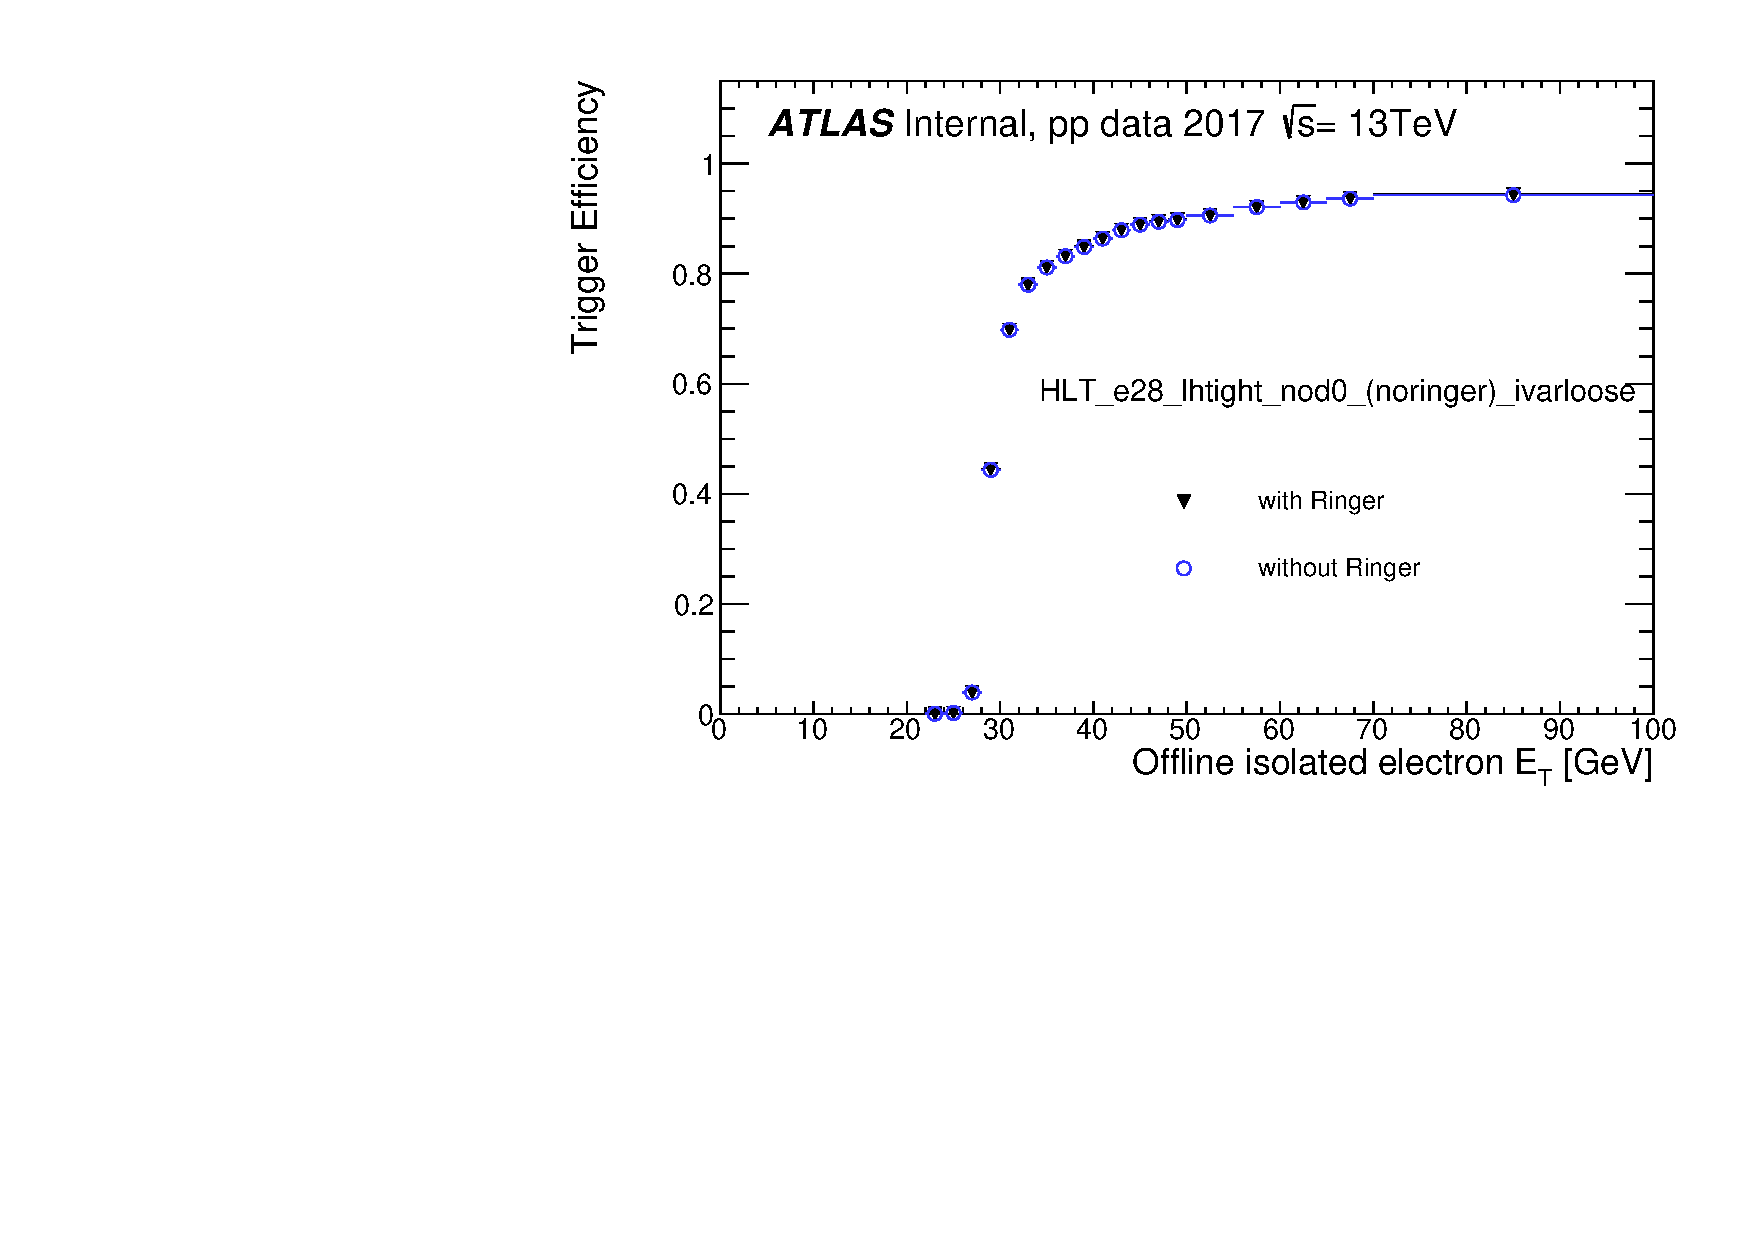
\includegraphics[width=\textwidth]{sections/operation/figures/efficiencies/eff_EGAM1_e28_ringer_and_noringer_2017_after_ts1_HLT_et.pdf}
  \caption{}%

  \end{subfigure}
  \hfill
  %\hspace{0.01\textwidth}
  \begin{subfigure}[c]{.48\textwidth}
  \centering
  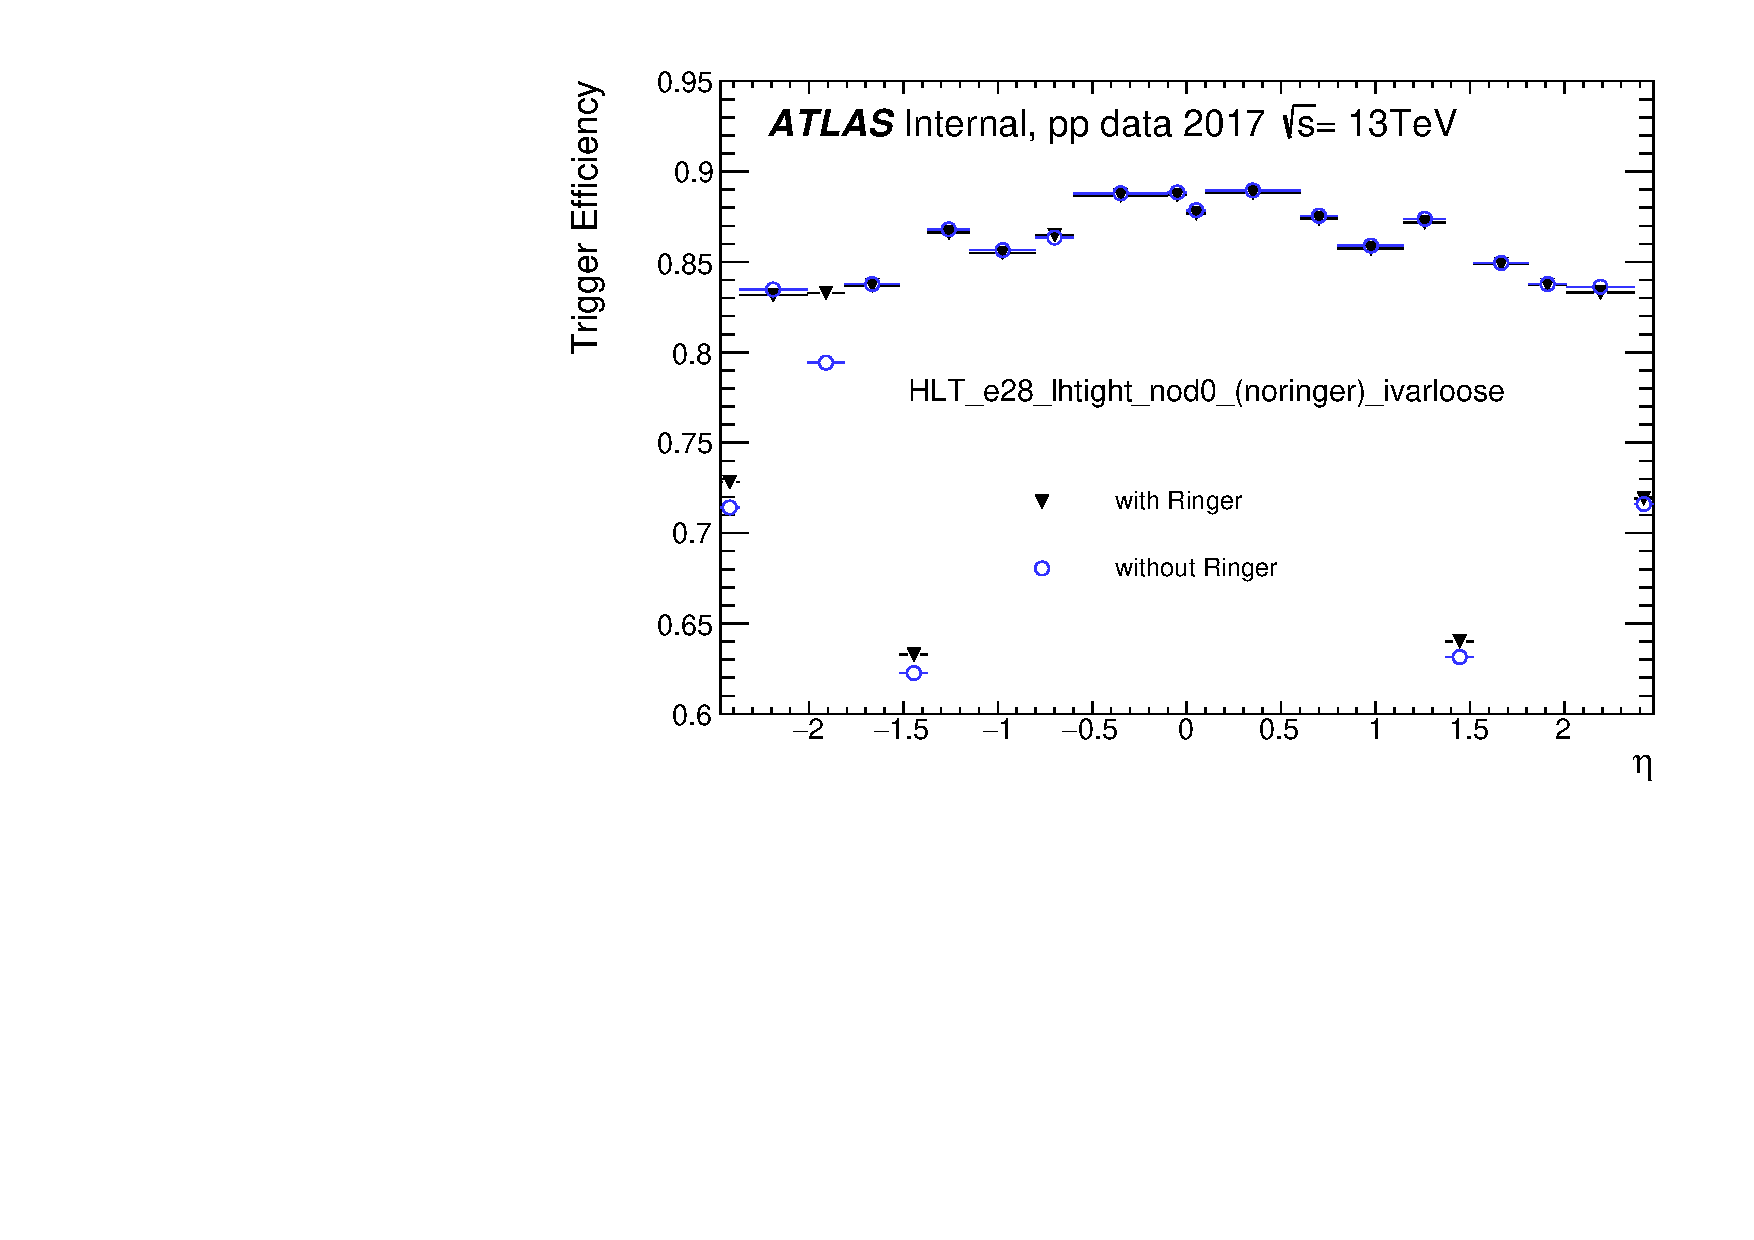
\includegraphics[width=\textwidth]{sections/operation/figures/efficiencies/eff_EGAM1_e28_ringer_and_noringer_2017_after_ts1_HLT_eta.pdf}
  \caption{}%
  %\label{fig:e28_comp_eta}
  \end{subfigure} \\
  \begin{subfigure}[c]{.48\textwidth}
  \centering
  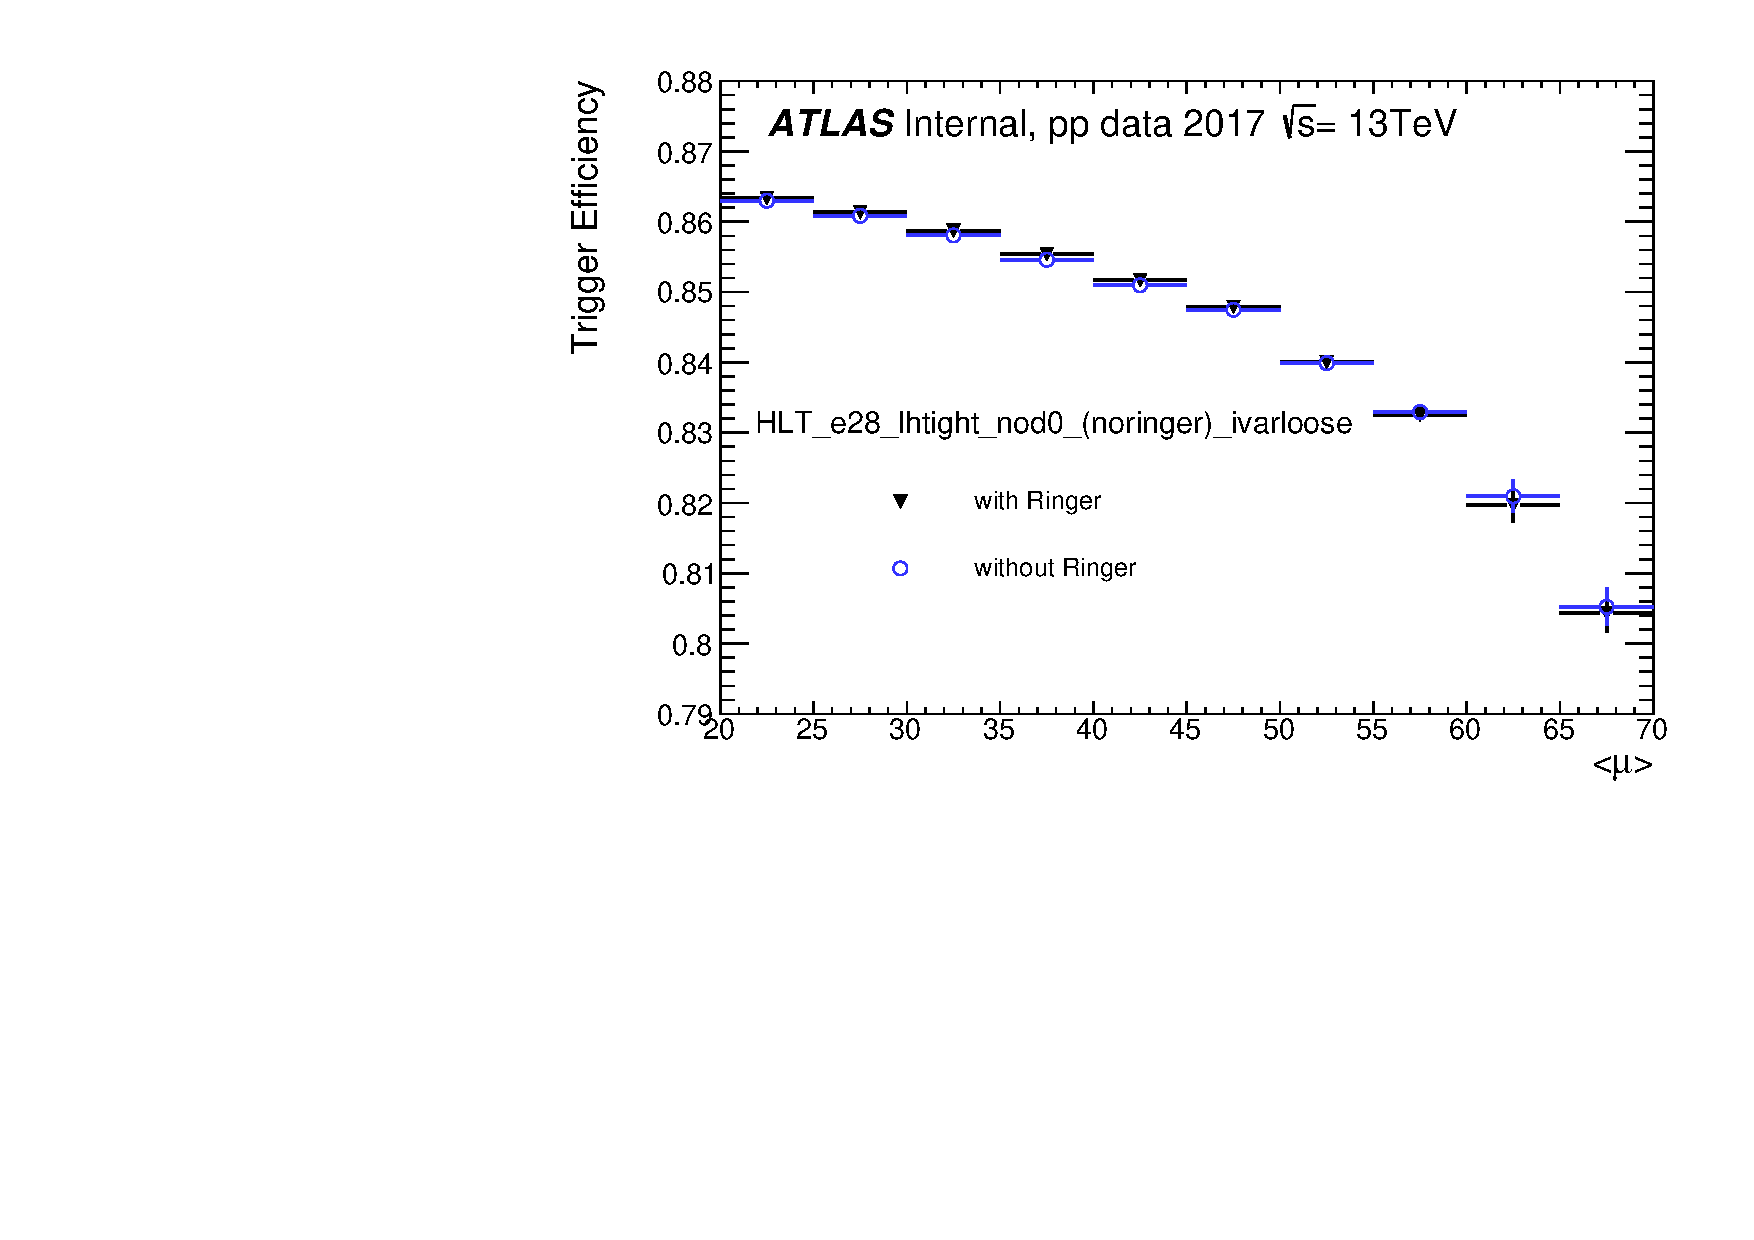
\includegraphics[width=\textwidth]{sections/operation/figures/efficiencies/eff_EGAM1_e28_ringer_and_noringer_2017_after_ts1_HLT_mu.pdf}
  \caption{}%
  \label{fig:e28_comp_mu}
  \end{subfigure}
  \caption{\label{fig:e28_triggers}HLT electron efficiency as a function of \et{}
    (a), \eta{} (b) and \avgmu{} (c) for the duplicated single electron trigger
    requiring $\et{} > \SI{28}{\GeV}$ and \tight{} selection with and without the
    \rnn{} algorithm. Efficiencies are measured employing 2017 data collected
    after TS1.}
  \end{center}
\end{figure}
  
\begin{figure}[h!tb]
  \begin{center}
  \begin{subfigure}[c]{.48\textwidth}
  \centering
  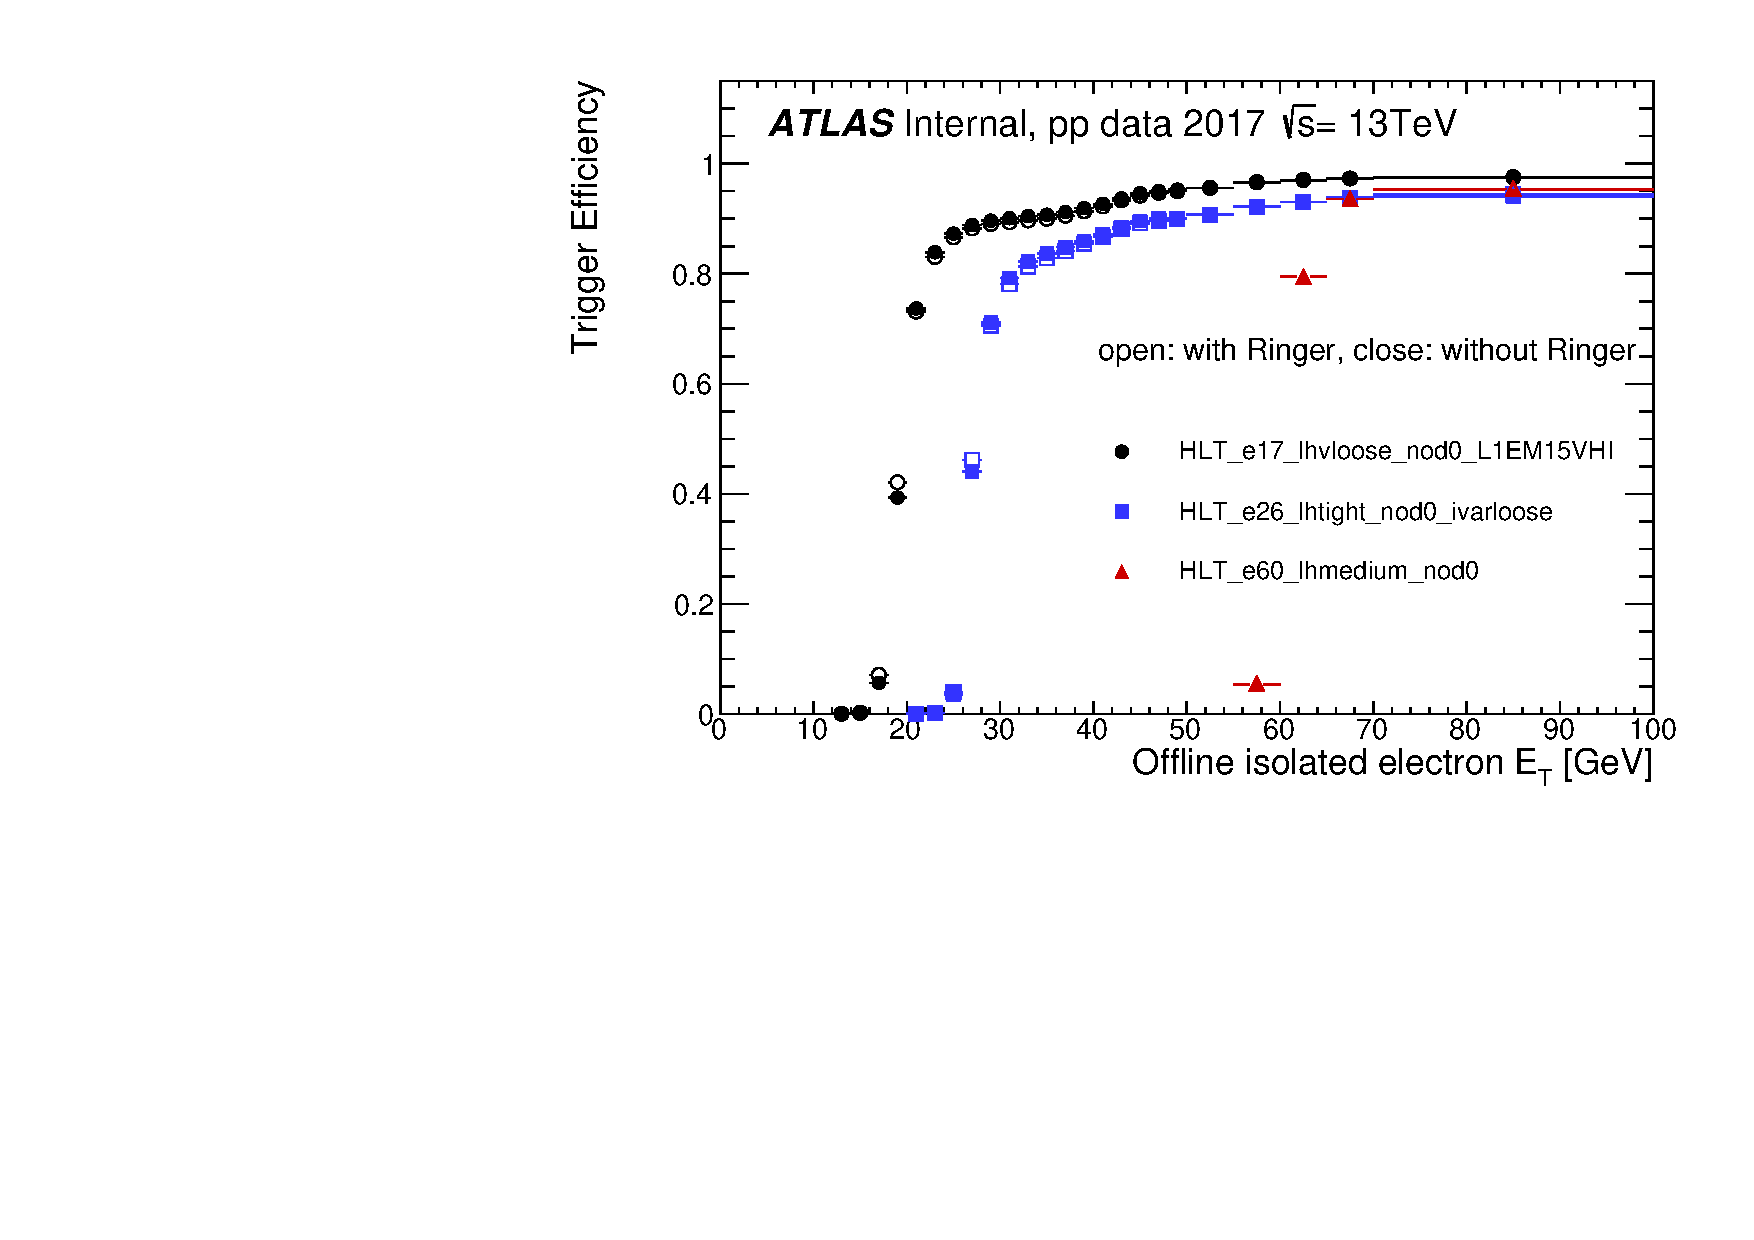
\includegraphics[width=\textwidth]{sections/operation/figures/efficiencies/eff_EGAM1_e17_e26_e60_2017_before_and_after_ts1_et.pdf}
  \caption{}%
  \end{subfigure}
  \hfill
  %\hspace{0.01\textwidth}
  \begin{subfigure}[c]{.48\textwidth}
  \centering
  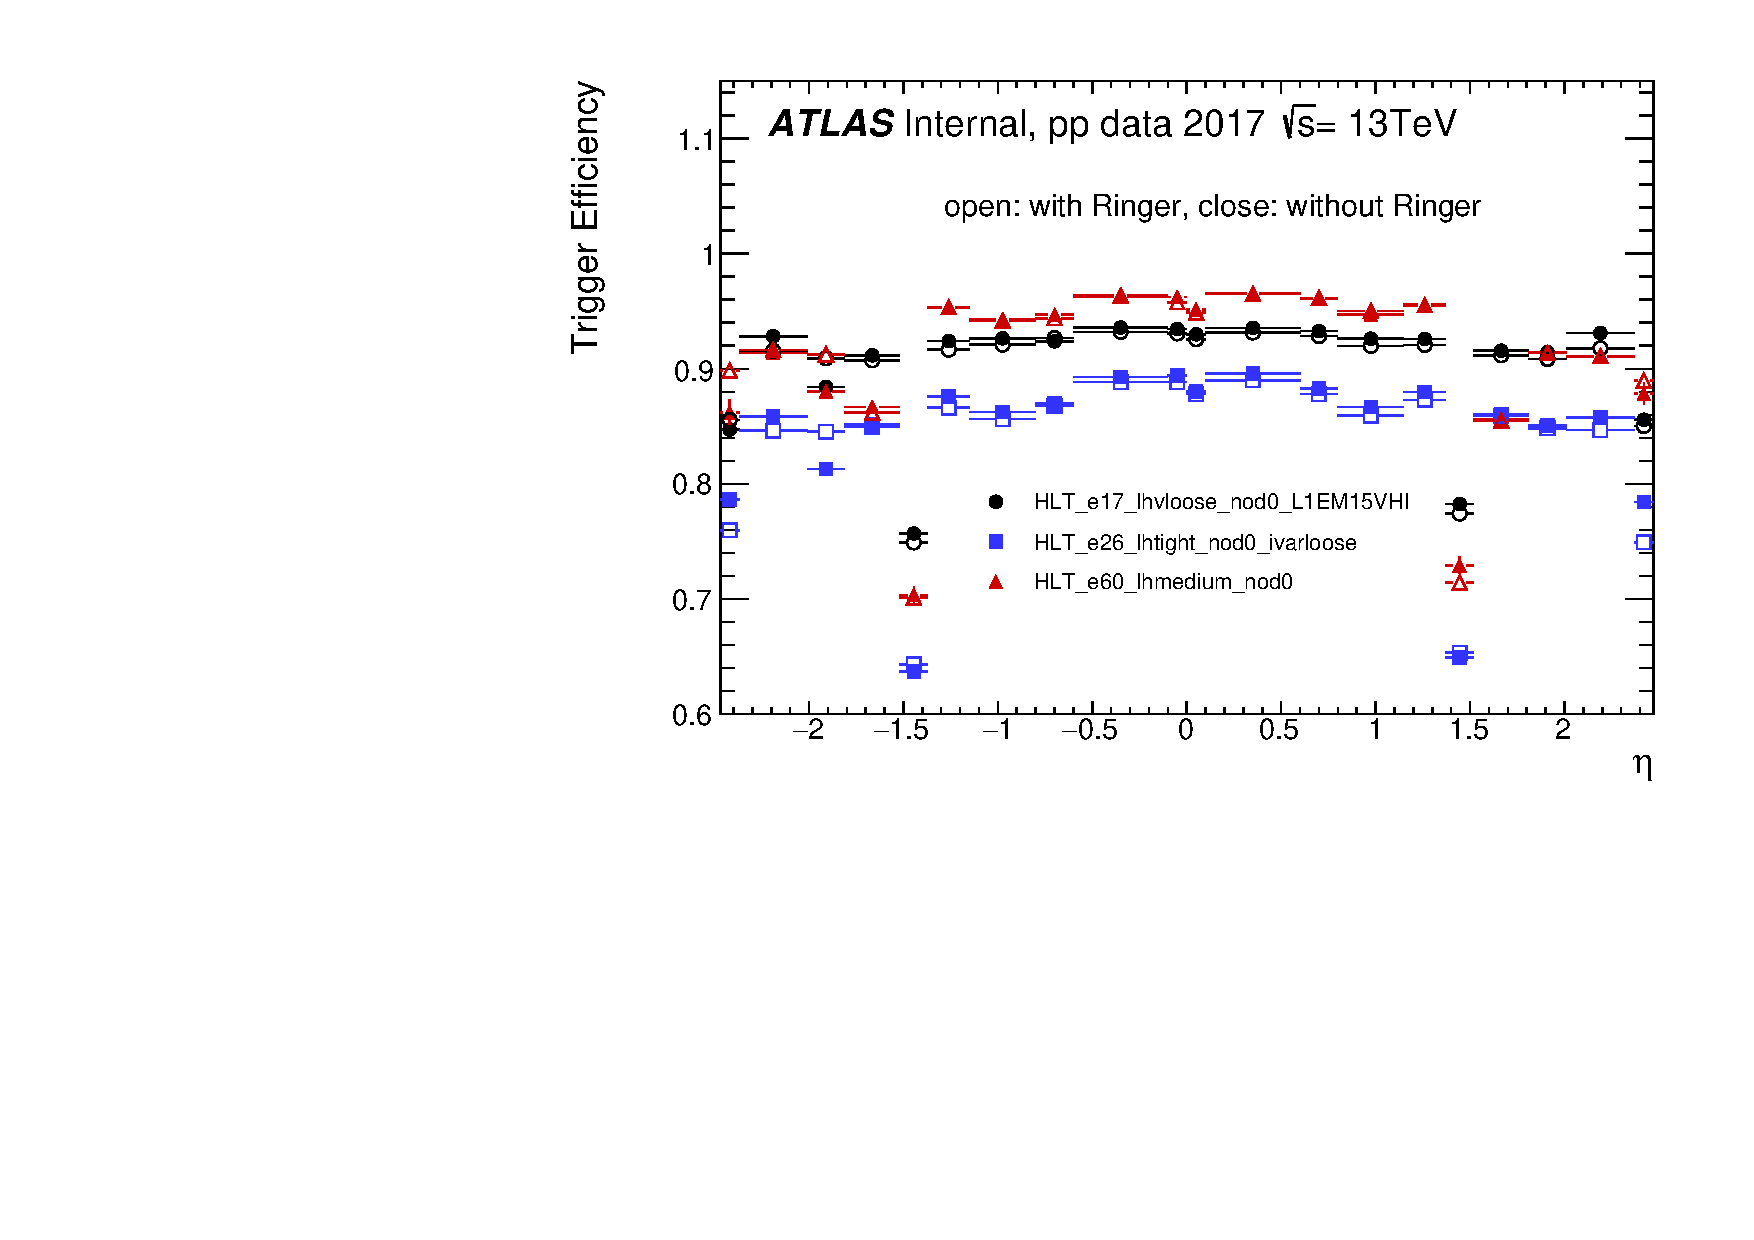
\includegraphics[width=\textwidth]{sections/operation/figures/efficiencies/eff_EGAM1_e17_e26_e60_2017_before_and_after_ts1_eta.pdf}
  \caption{}%
  \end{subfigure} \\
  \begin{subfigure}[c]{.48\textwidth}
  \centering
  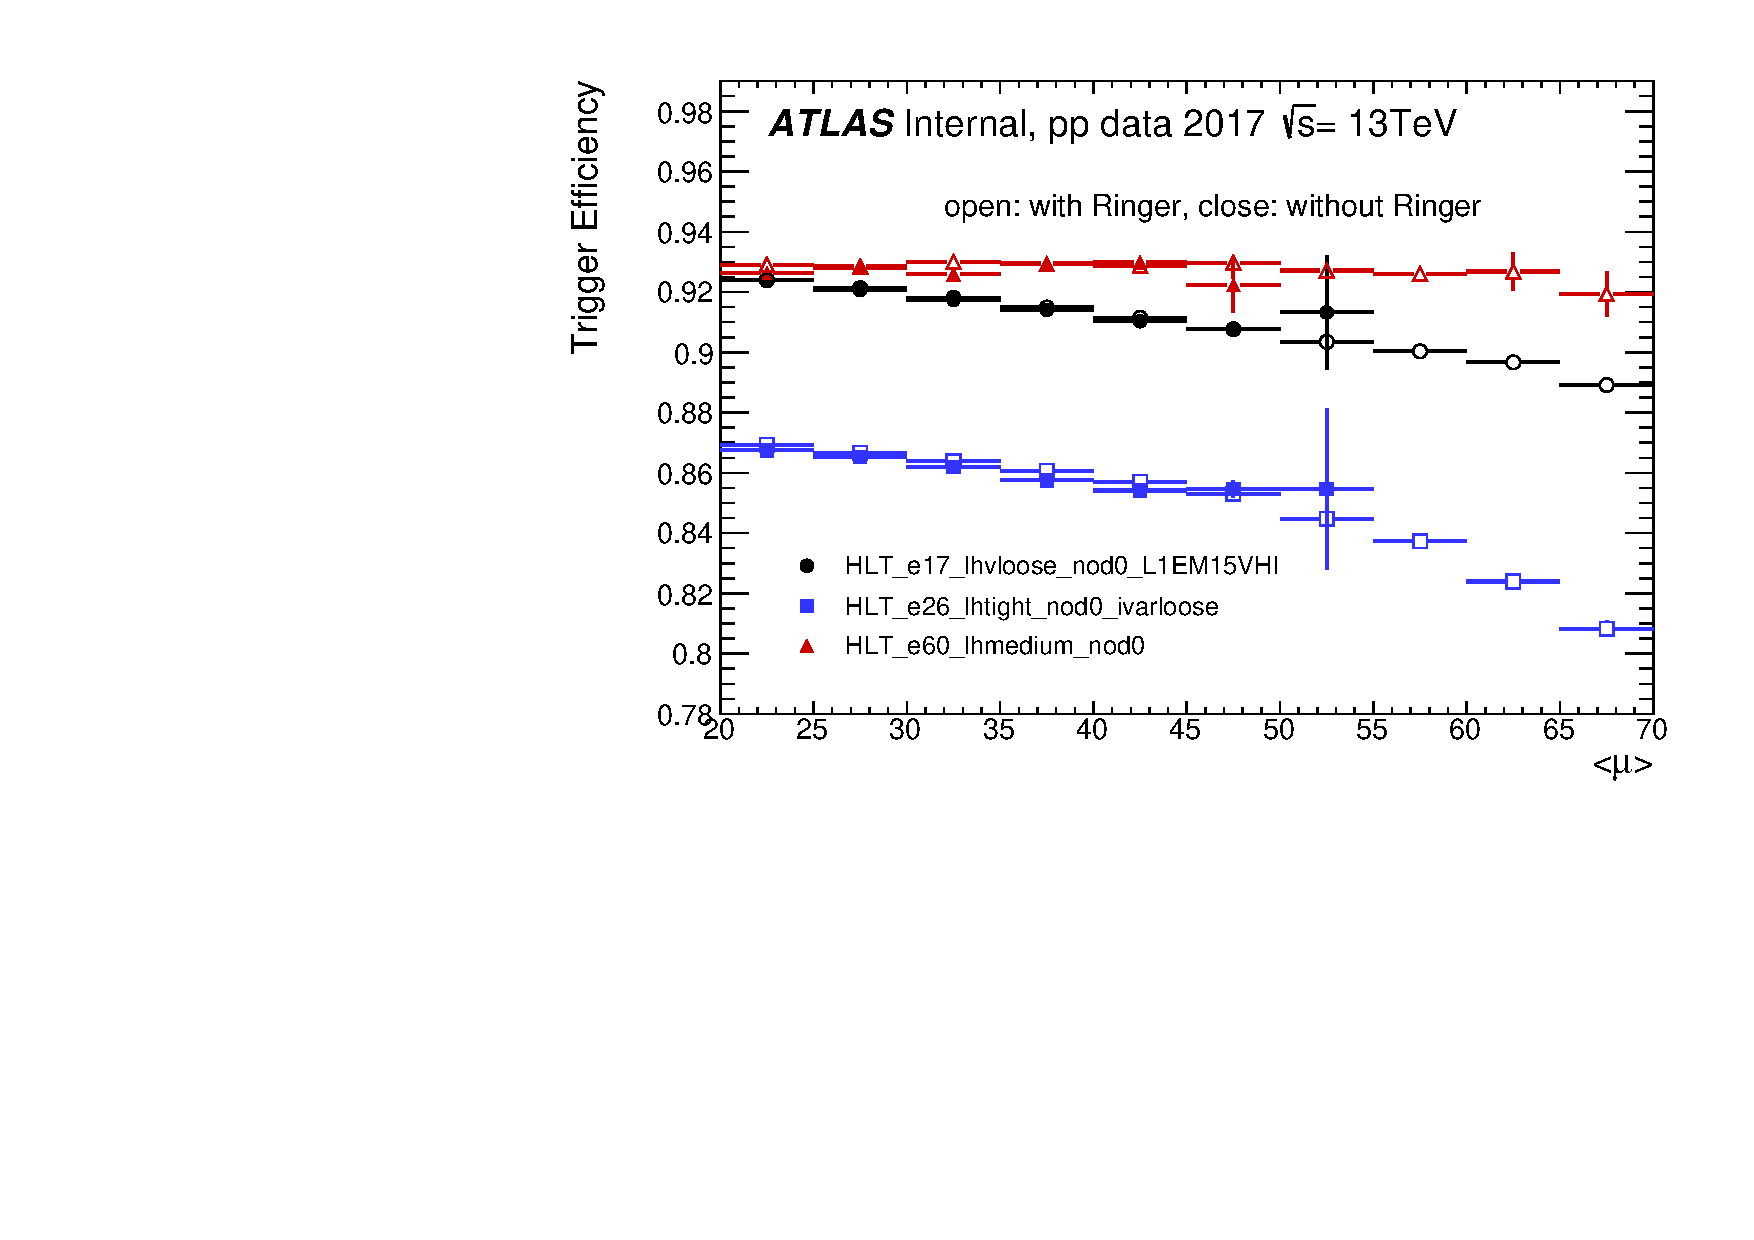
\includegraphics[width=\textwidth]{sections/operation/figures/efficiencies/eff_EGAM1_e17_e26_e60_2017_before_and_after_ts1_mu.pdf}
  \caption{}%
  \end{subfigure}
  %\hfill
  \caption{Efficiency of three single electron triggers as a function of
  \et (a), \eta (b) and \avgmu (c). Open (closed) markers contain
  the efficiency measurements on runs before (after) TS1, thus referring to
  triggers being executed without (with) the \rnn{} algorithm.
  }%
  \label{fig:2017_ts1}
  \end{center}
\end{figure}


By contrasting the behavior of the duplicated trigger using fake electron data,
it becomes clear the power of the \rnn{} algorithm. An overall reduction factor of
the fake rate by 13.75 is achieved. It can be seen in
Figure~\ref{fig:e28_triggers_fake} that the improvement is similar for all
regions in the evaluated variables, particularly interesting when
considering the low \et{} and the end-cap regions.




\begin{figure}[h!tb]
  \begin{center}
  \begin{subfigure}[c]{.48\textwidth}
  \centering
  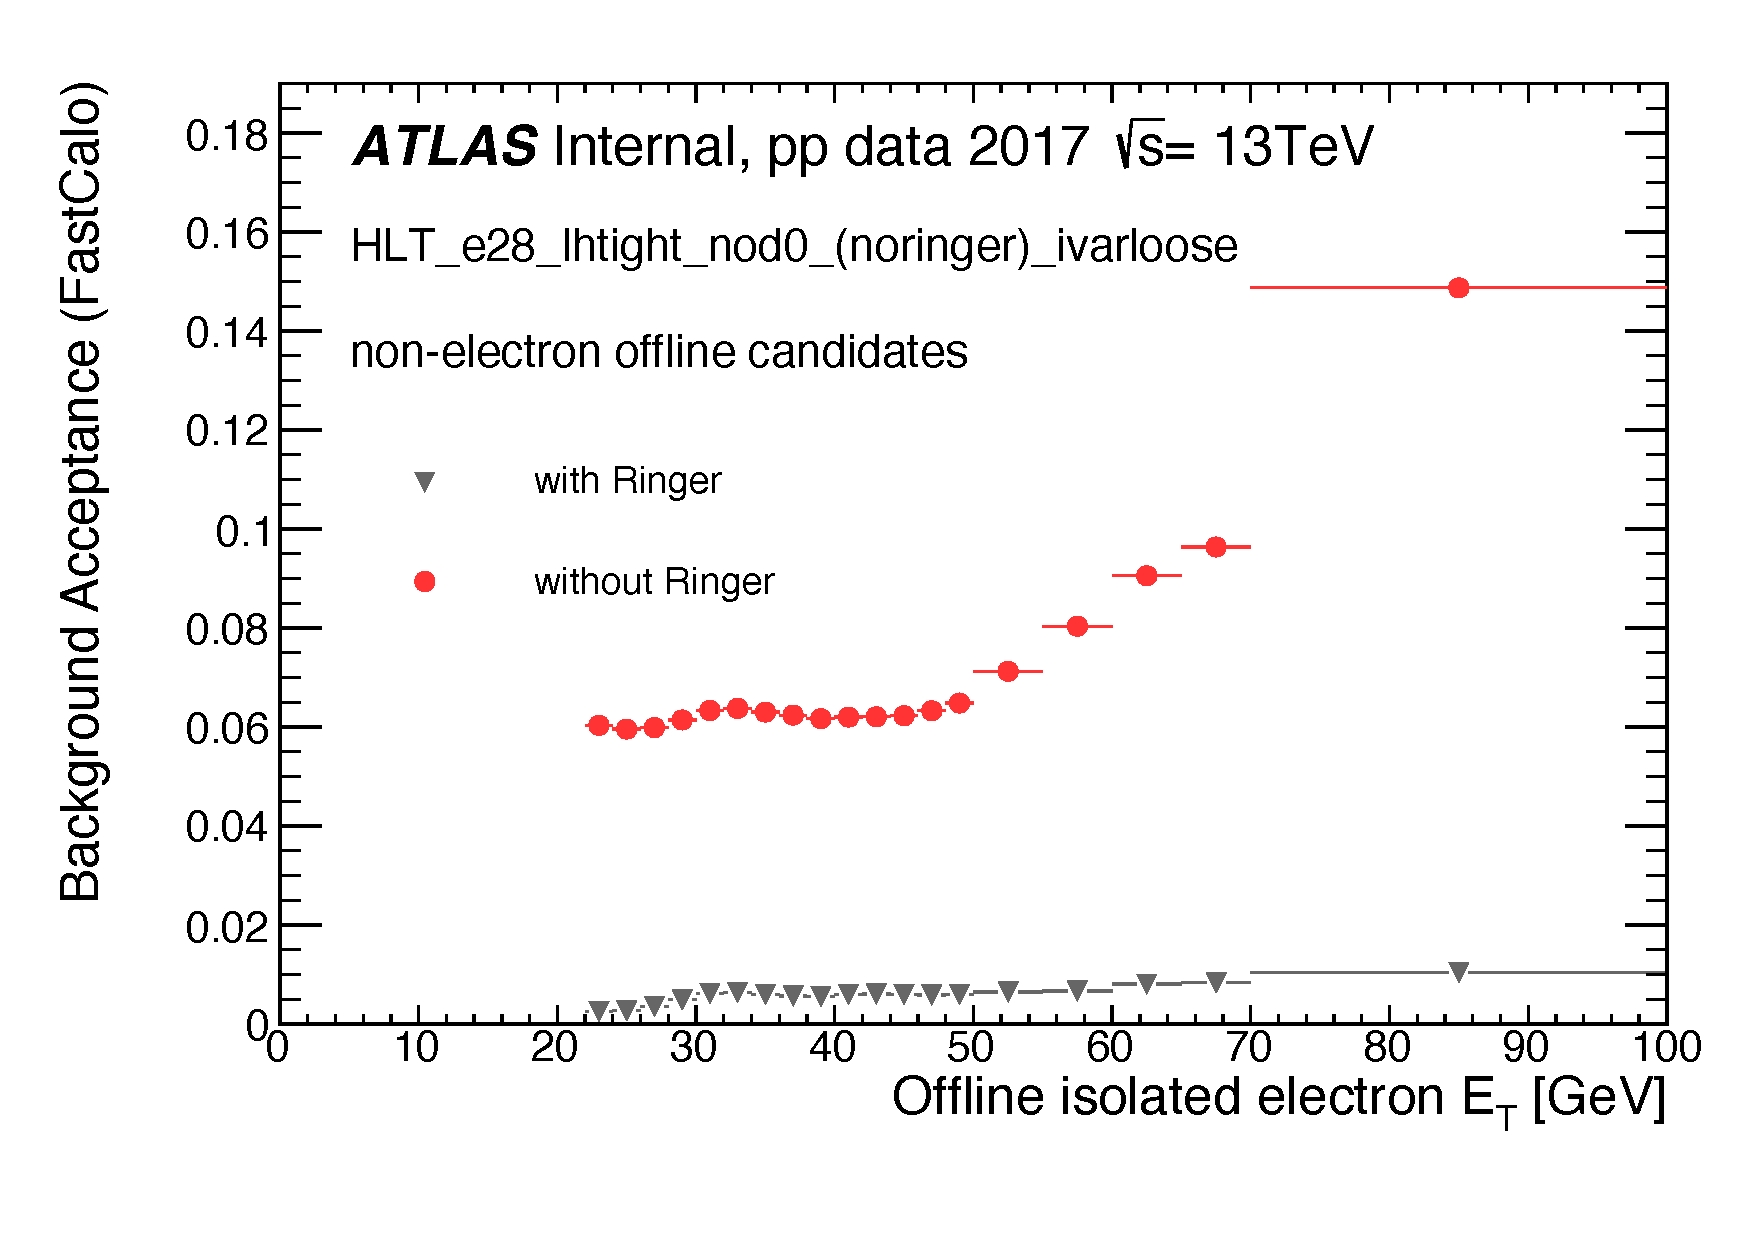
\includegraphics[width=\textwidth]{sections/operation/figures/efficiencies/eff_EGAM7_e28_ringer_and_noringer_2017_after_ts1_L2Calo_et.pdf}
  %\label{fig:e28_comp_et_fake}
  \caption{}
  \end{subfigure}
  \hfill
  %\hspace{0.01\textwidth}
  \begin{subfigure}[c]{.48\textwidth}
  \centering
  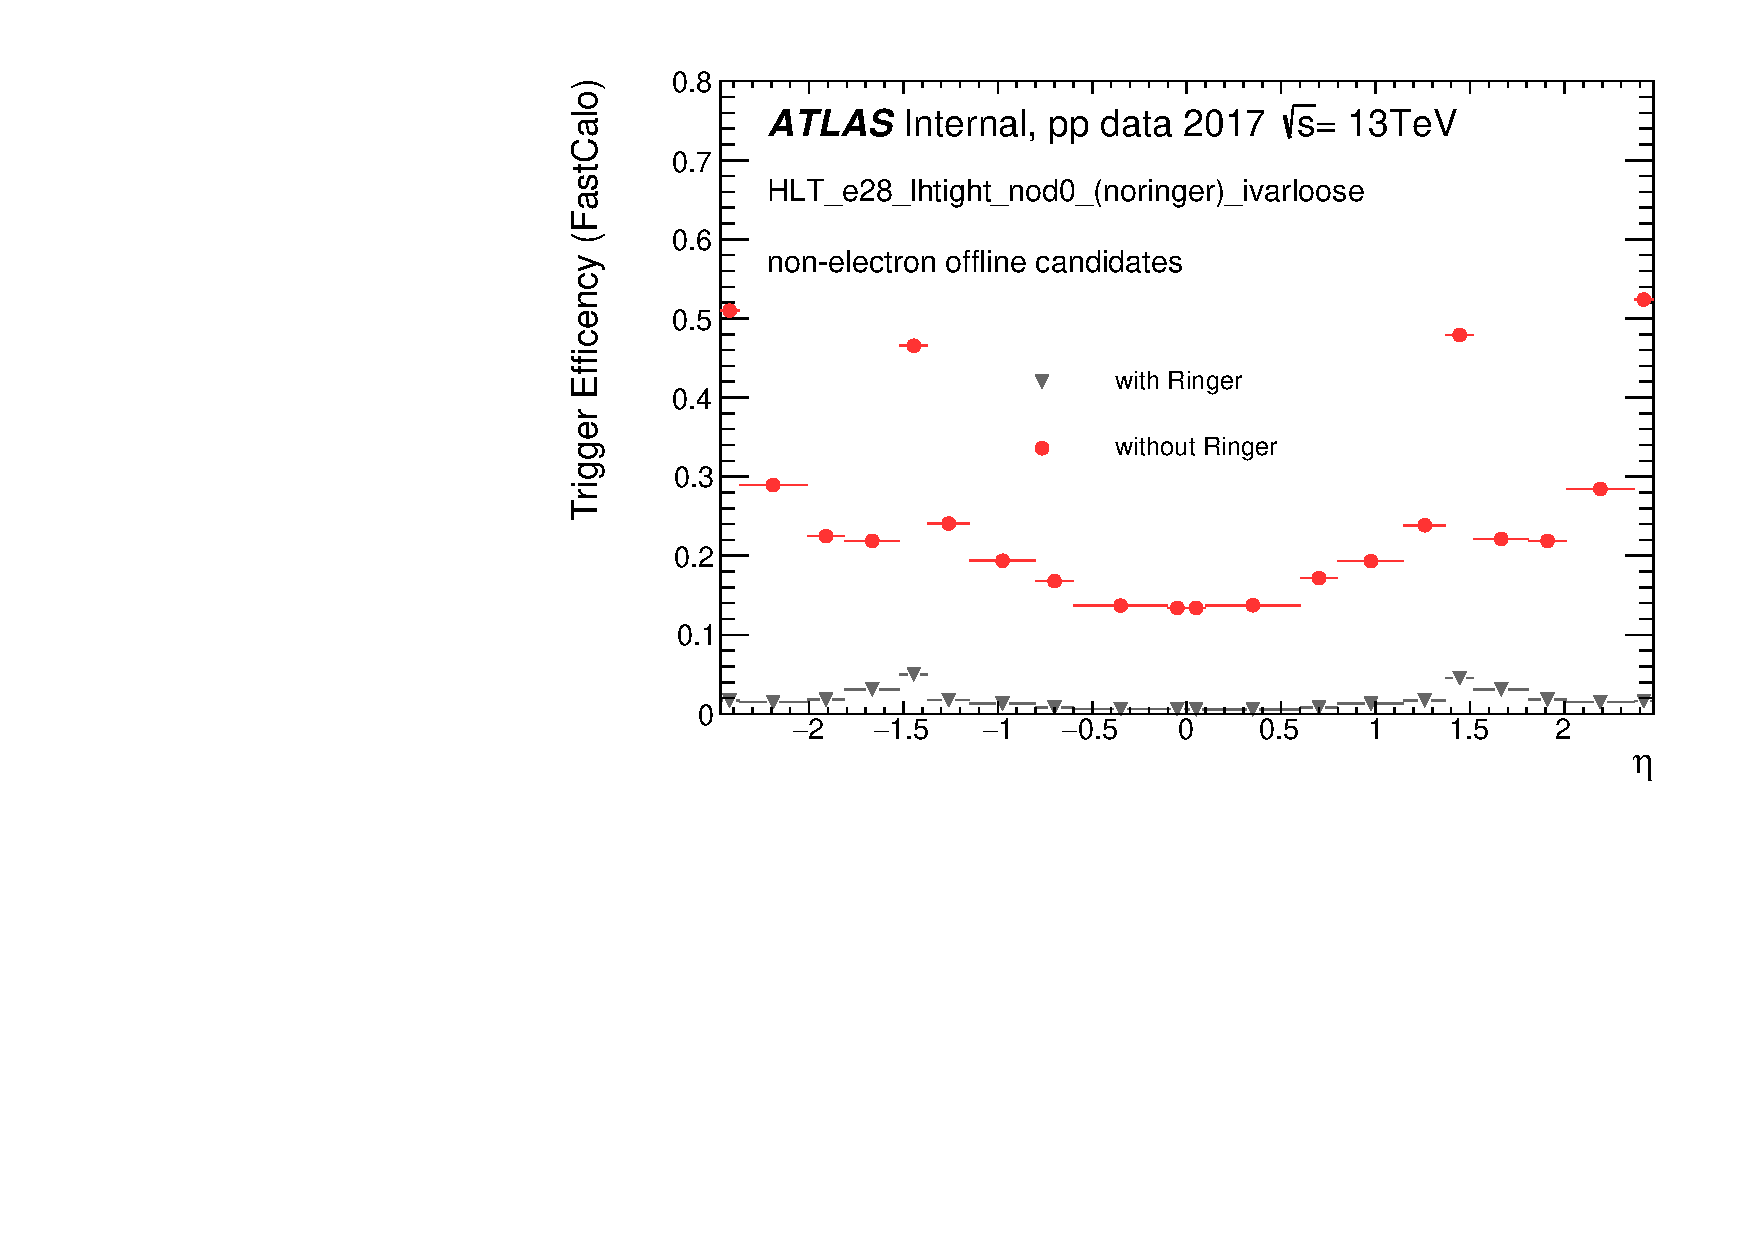
\includegraphics[width=\textwidth]{sections/operation/figures/efficiencies/eff_EGAM7_e28_ringer_and_noringer_2017_after_ts1_L2Calo_eta.pdf}
  %\label{fig:e28_comp_eta_fake}
  \caption{}
  \end{subfigure}\\
  \begin{subfigure}[c]{.48\textwidth}
  \centering
  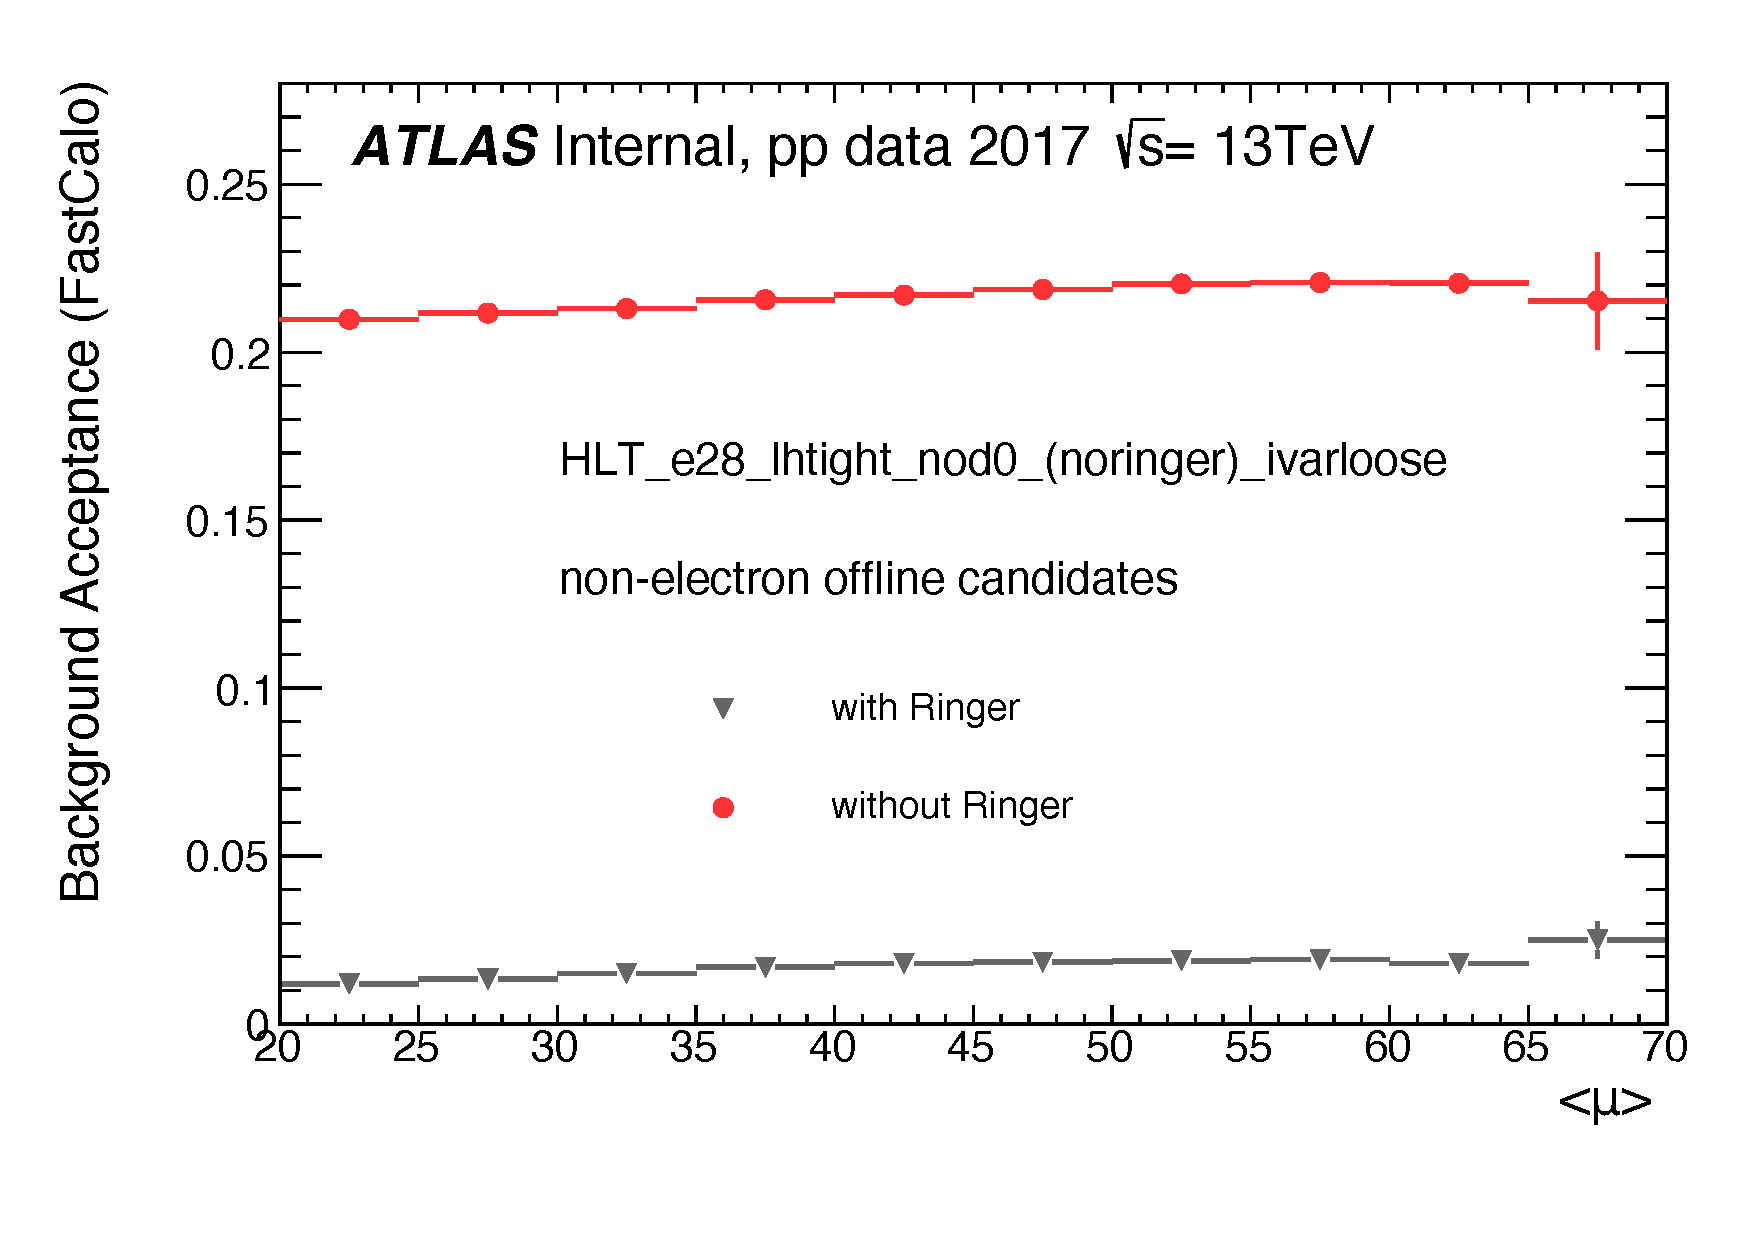
\includegraphics[width=\textwidth]{sections/operation/figures/efficiencies/eff_EGAM7_e28_ringer_and_noringer_2017_after_ts1_L2Calo_mu.pdf}
  %\label{fig:e28_comp_mu_fake}
  \caption{}
  \end{subfigure}
  %\hfill
  \caption{\label{fig:e28_triggers_fake} \fastcalo %\footnotemark{} 
  fake electron efficiency as a function of \et (a), \eta (b) and \avgmu (c) for the
  duplicated single electron trigger requiring $\et > \SI{28}{\GeV}$ and \tight
  selection with and without the \rnn{} algorithm. Efficiencies are measured
  employing 2017 data collected after TS1.}%
  
  \end{center}
\end{figure}



Besides the capability of improving early fake rejection, the usage of the
\rnn{} also contributed to reduce the final fake rate
(Figure~\ref{fig:e28_triggers_fake_hlt}) by a factor of 2, mostly coming from
the end-cap and crack regions. %This fake rate reduction when measured with
%respect to the offline electron selection does not seem to have impacted in the
%output rate (see Appendix~\ref{ssec:primary_rate_wrt_luminosity})\footnote{This
%  can provide some indication that measuring background efficiencies with
%respect to the offline may not be the best approach.}, but may have
%contributed to reduce signal contamination in physics analyses.

\begin{figure}[h!tb]
\begin{center}
\begin{subfigure}[c]{.48\textwidth}
\centering
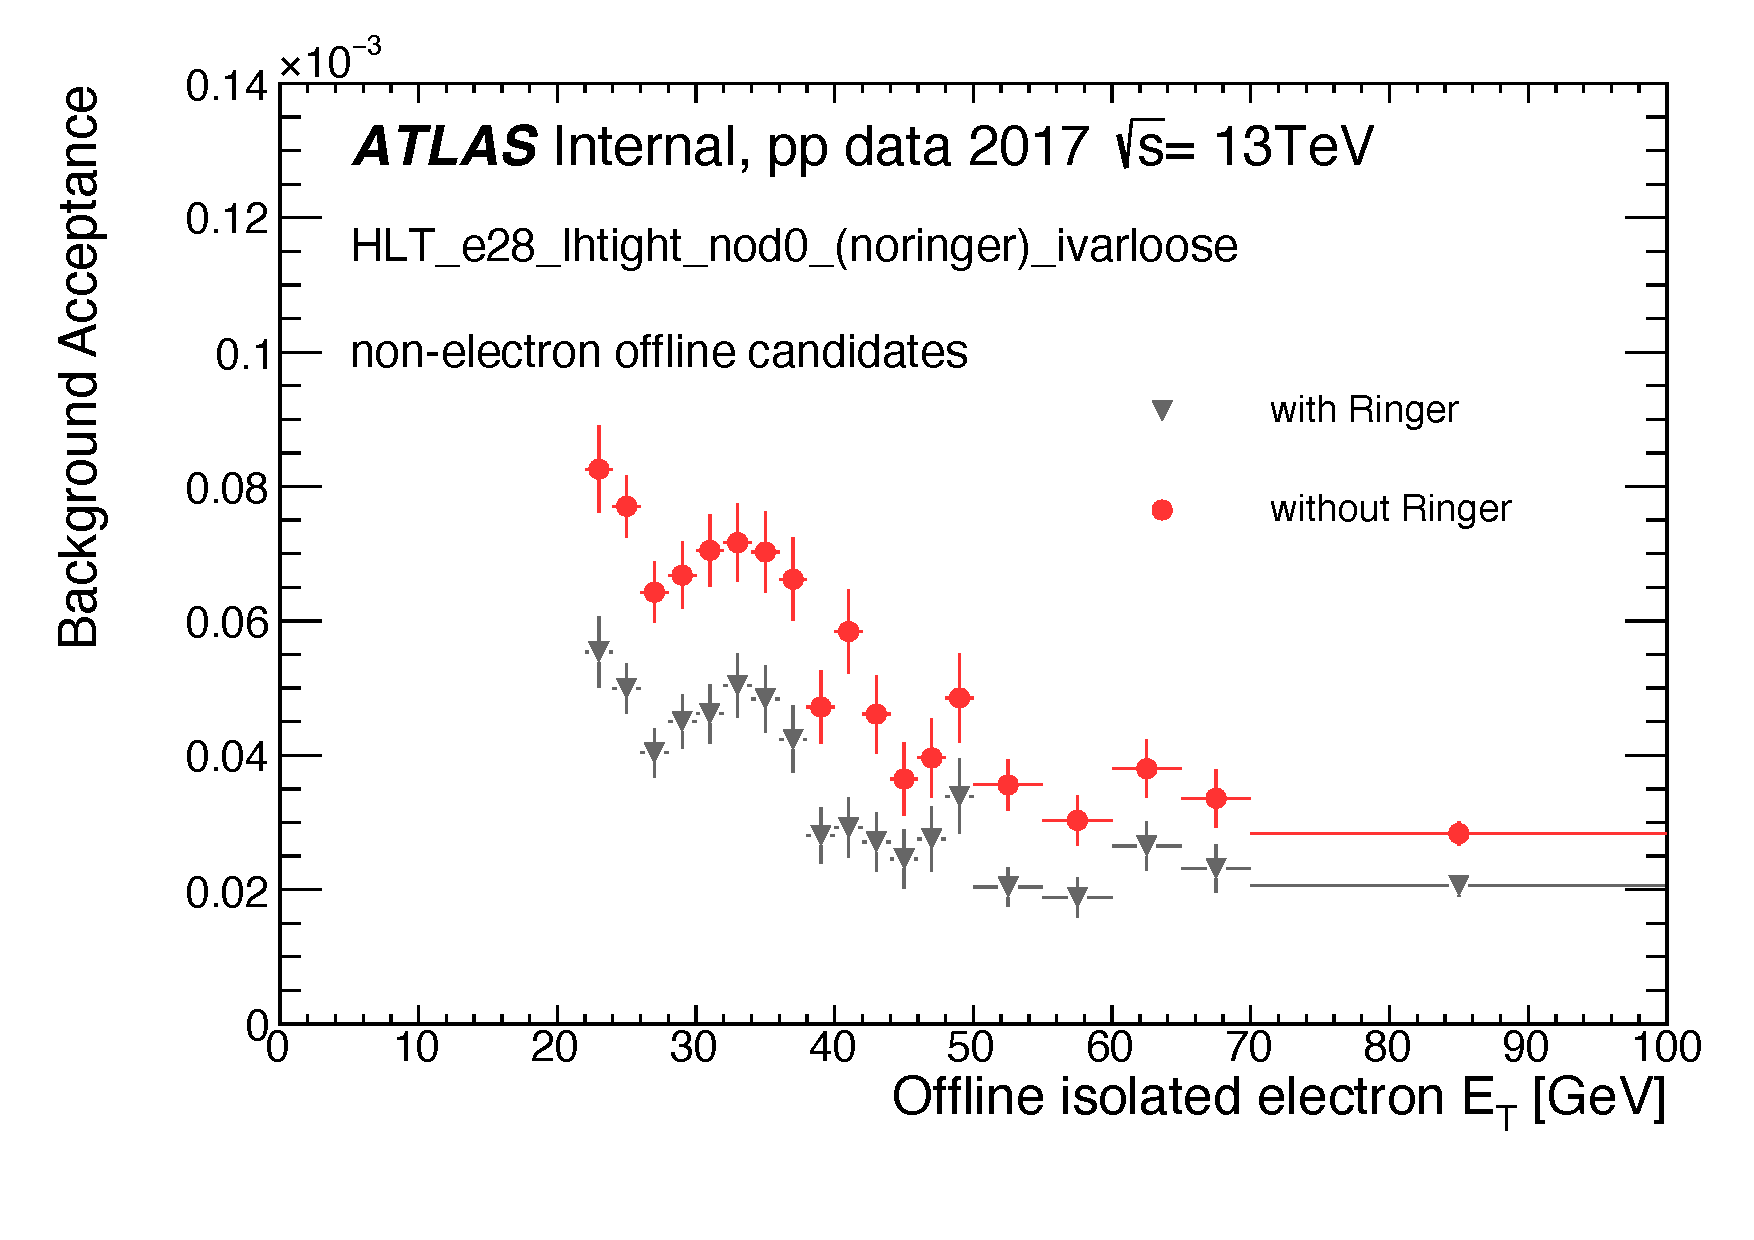
\includegraphics[width=\textwidth]{sections/operation/figures/efficiencies/eff_EGAM7_e28_ringer_and_noringer_2017_after_ts1_et.pdf}
\caption{}
\end{subfigure}
\hfill
%\hspace{0.01\textwidth}
\begin{subfigure}[c]{.48\textwidth}
\centering
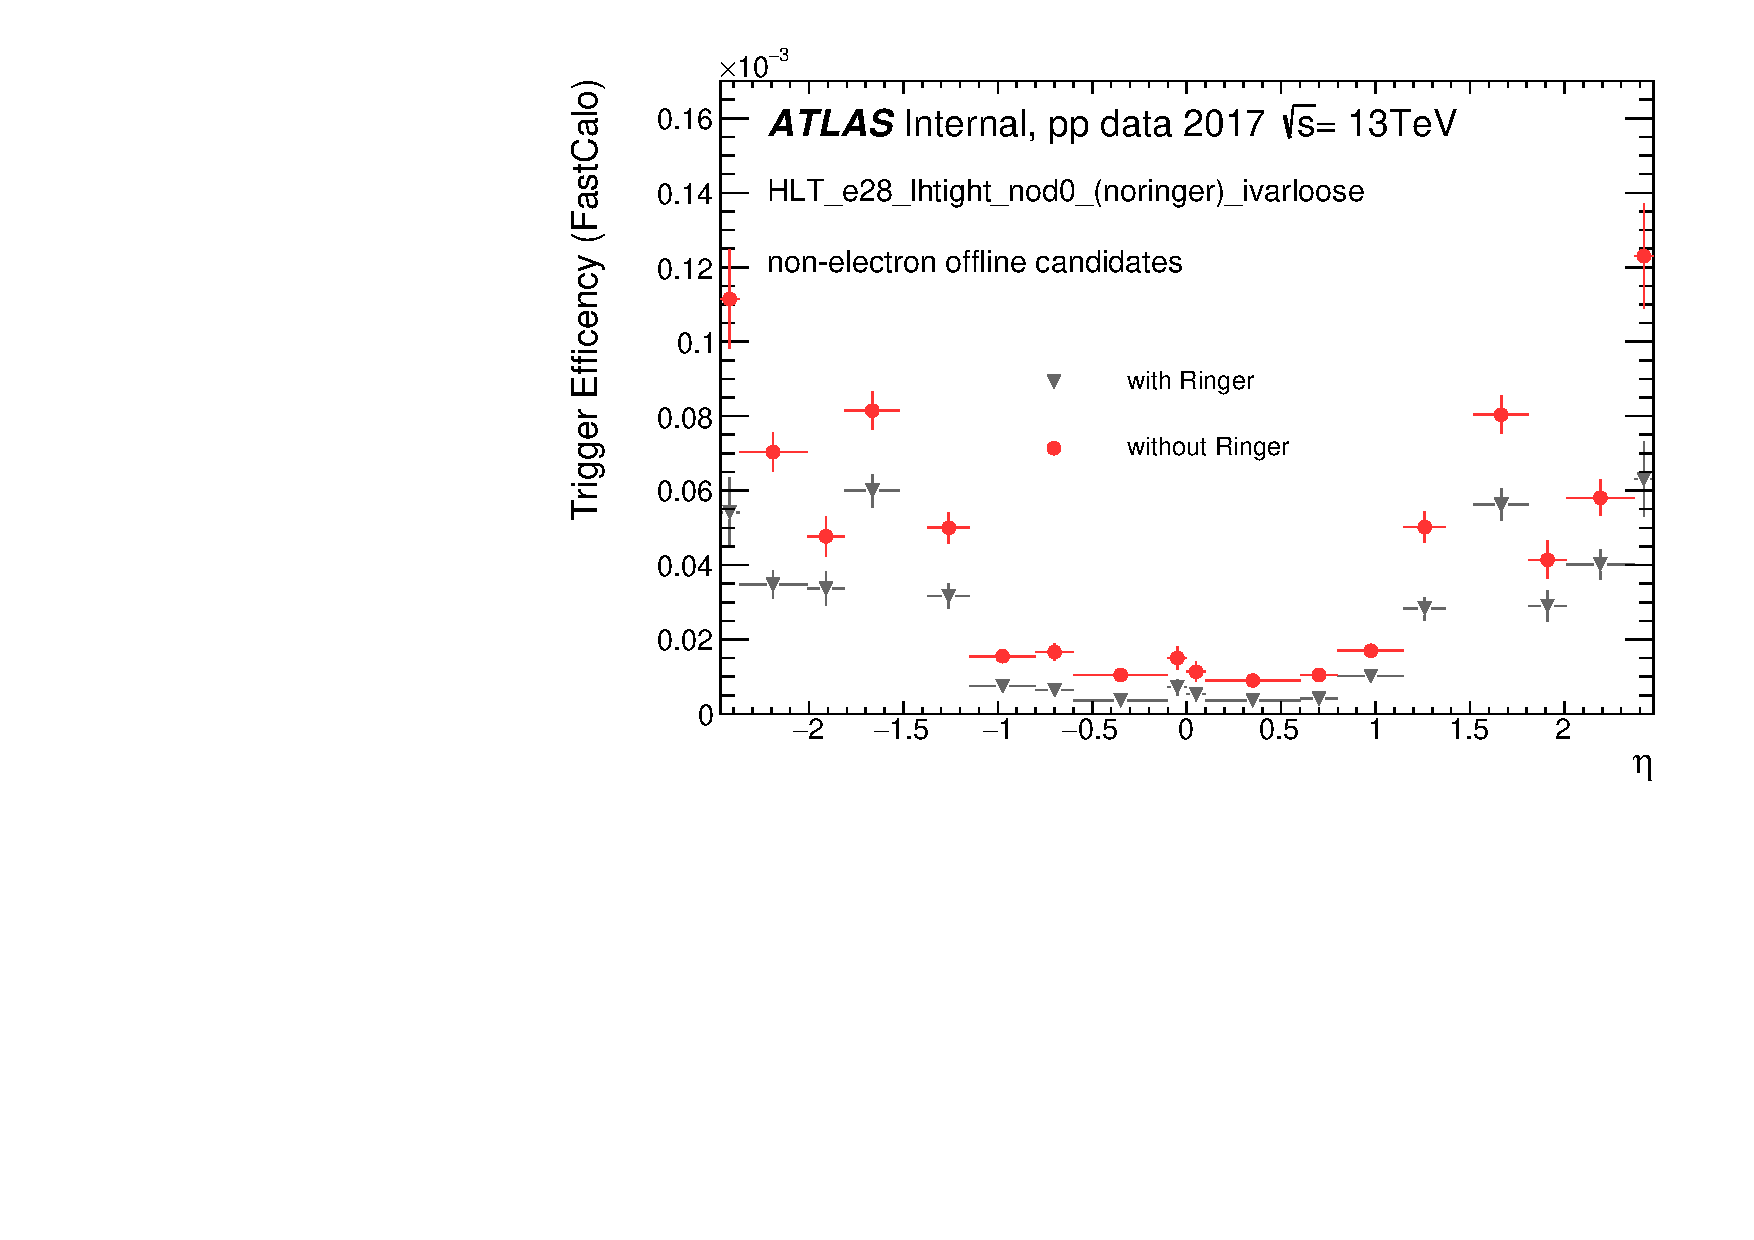
\includegraphics[width=\textwidth]{sections/operation/figures/efficiencies/eff_EGAM7_e28_ringer_and_noringer_2017_after_ts1_eta.pdf}
\caption{}
\end{subfigure} \\
\begin{subfigure}[c]{.48\textwidth}
\centering
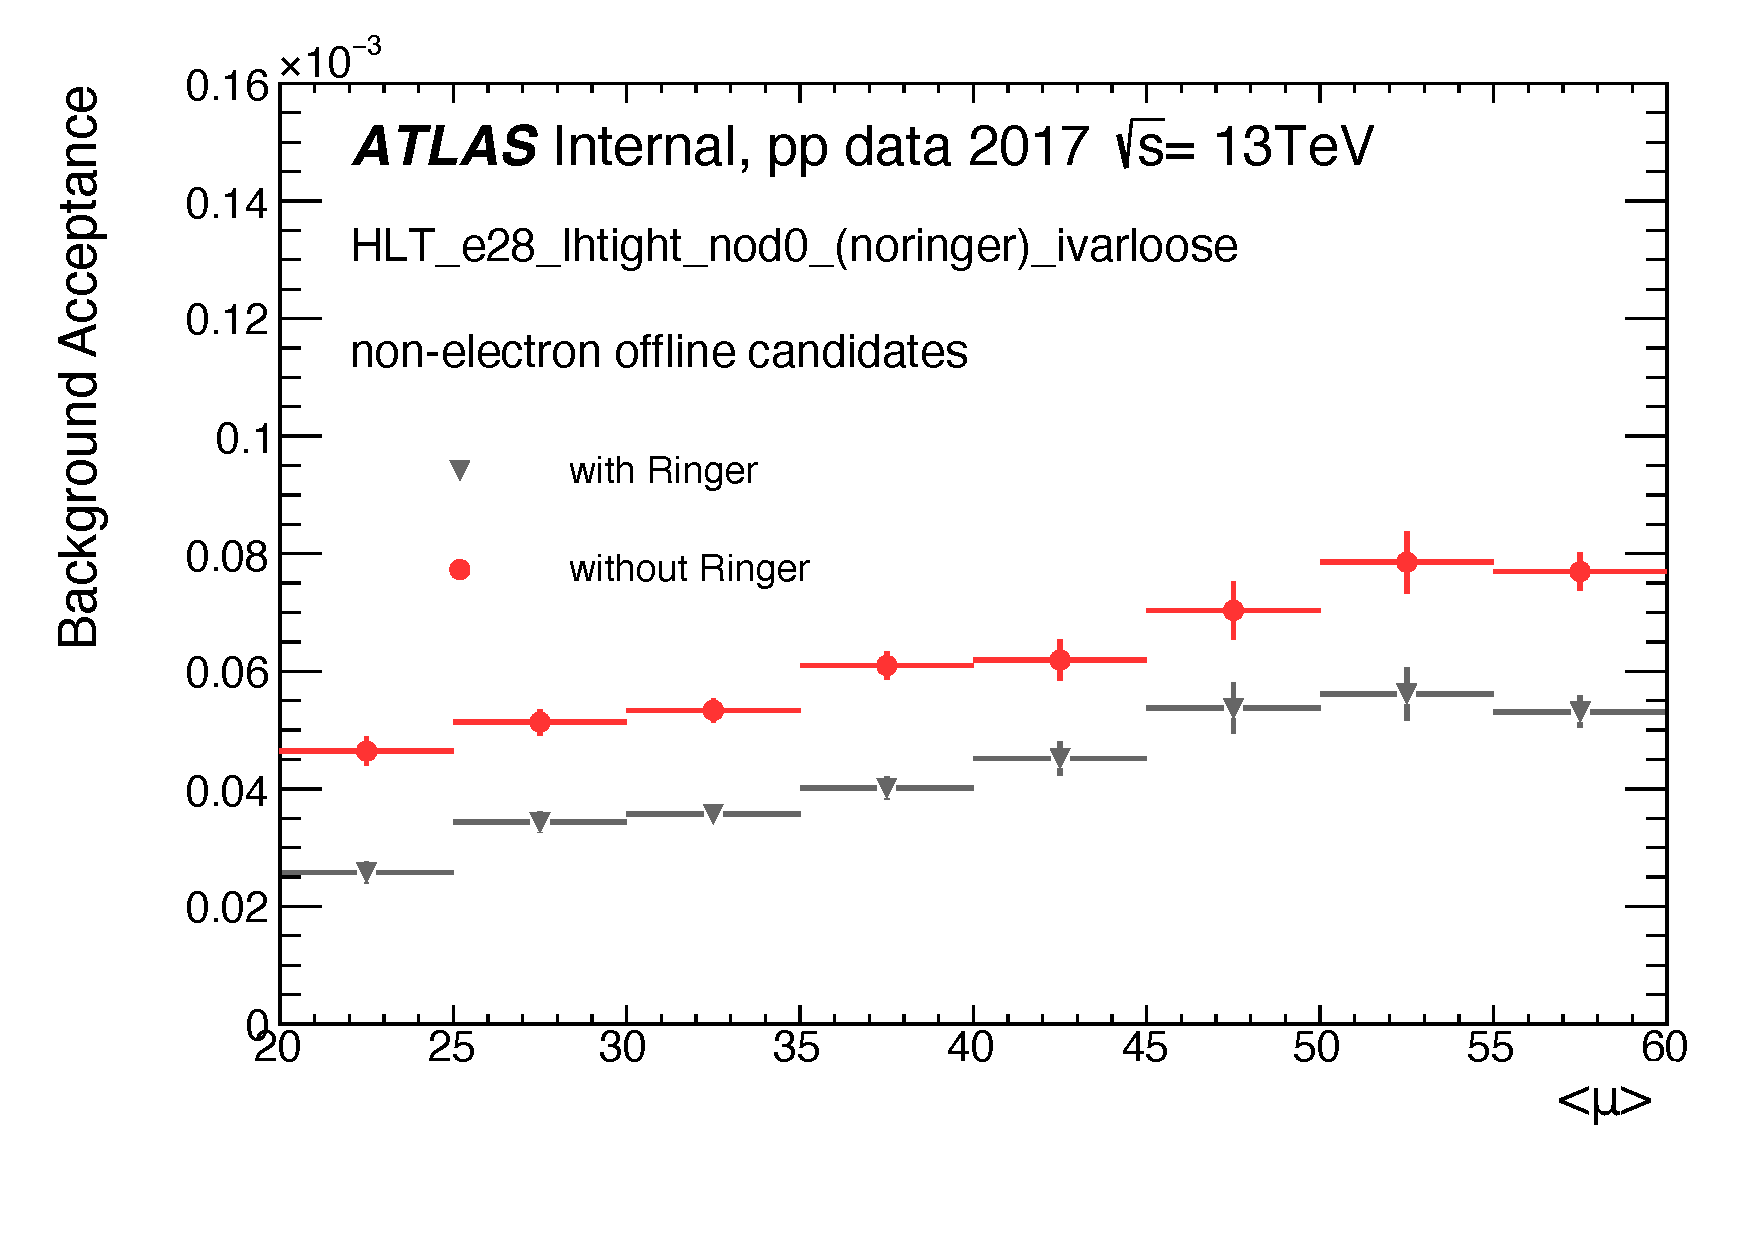
\includegraphics[width=\textwidth]{sections/operation/figures/efficiencies/eff_EGAM7_e28_ringer_and_noringer_2017_after_ts1_mu.pdf}
\caption{}
\end{subfigure}
\caption{HLT fake electron efficiency as a function of \et (a), \eta (b) and
\avgmu (c) for the duplicated single electron trigger requiring $\et >
\SI{28}{\GeV}$ and \tight selection with and without the \rnn{} algorithm.
Efficiencies are measured employing 2017 data collected after TS1.}%
\label{fig:e28_triggers_fake_hlt}
\end{center}
\end{figure}


\FloatBarrier

\section{2018 Operation}\label{ssec:2018_ringer_operation}

In 2018, the \rnn{} operated with a new tune based on collision data
(Section~\ref{ssec:2018}). It was also the case for the final HLT
selection\footnote{One exception was the \medium{} selection, where the HLT
likelihood selection operated in 2018 with the same 2017 tune.}. For the
lowest-transverse energy-threshold unprescaled trigger, an efficiency
improvement of at least one percentage point in central value is observed when
comparing both periods, resulting from a better operation in all selection
steps, but, in particular, this is due to improvements from the likelihood tunes in the period.

Despite maintaining high electron efficiency, it was observed a small reduction in fake acceptance at \fastcalo{} for some unprescaled triggers in comparison with 2017 after TS1. For the lowest-transverse energy-threshold it is observed a reduction factor by 1.19. On the other hand, for the highest-transverse energy trigger, a reduction factor by 1.69 was achieved.


